\documentclass[12pt,a4paper]{article}
\usepackage{amsmath, amssymb, geometry, booktabs, xcolor, hyperref,
            listings, pgfplots, tcolorbox, enumitem, fancyhdr, tikz, array}
\geometry{margin=2.5cm}
\pgfplotsset{compat=1.18}
\tcbuselibrary{skins, breakable}

% --------------- tcolorbox environments ---------------
\newtcolorbox{curiositybox}[1]{colback=yellow!10, colframe=orange!80!black,
  fonttitle=\bfseries, title=#1, breakable}
\newtcolorbox{infobox}[1]{colback=blue!5, colframe=blue!60!black,
  fonttitle=\bfseries, title=#1, breakable}
\newtcolorbox{mistakebox}[1]{colback=red!5, colframe=red!60!black,
  fonttitle=\bfseries, title=#1, breakable}
\newtcolorbox{learnbox}[1]{colback=green!5, colframe=green!60!black,
  fonttitle=\bfseries, title=#1, breakable}

% --------------- lstlisting ---------------
\lstset{language=Python, basicstyle=\ttfamily\small,
        keywordstyle=\color{blue}, commentstyle=\color{gray},
        stringstyle=\color{orange}, showstringspaces=false,
        numbers=left, numberstyle=\tiny, breaklines=true, frame=single}

% --------------- fancyhdr ---------------
\pagestyle{fancy}
\fancyhf{}
\lhead{Topic 01: Inverse Laplace Transform}
\rhead{Unit V --- Inverse Laplace Transforms}
\cfoot{\thepage}

% --------------- title ---------------
\title{Topic 01: Inverse Laplace Transform \\ \large Unit V --- Inverse Laplace Transforms}
\author{\\
JNTUA College of Engineering (Autonomous) ATP}
\date{}

% ======================================================
\begin{document}
\maketitle
\tableofcontents
\newpage

% ======================================================
\section{Opening Hook}

\begin{curiositybox}{Hook}
All of Unit IV was about the forward journey: $f(t) \to F(s)$.
The Laplace Transform is a machine that converts time-domain functions into
s-domain representations. But what about the return trip? You solve an
algebraic equation in the s-domain and get $Y(s)$. To get the actual solution
$y(t)$, you need to invert --- to press ``undo'' on the Laplace machine.
The Inverse Laplace Transform is that undo button. This topic shows you
exactly how it works, and gives you the standard inverse table that mirrors
everything you learned in Unit IV.
\end{curiositybox}

% ======================================================
\section{Why This Topic Exists}

Before we begin, here is the honest answer to why you are reading this.
Solving ordinary differential equations via Laplace transforms is a
two-stage process: convert the ODE to an algebraic equation in $s$, solve for
$Y(s)$, then \emph{invert} to recover $y(t)$. Without the inverse step, you
stop halfway. The forward transform gets you to $Y(s)$; the inverse transform
brings you home to $y(t)$.

\vspace{6pt}
\begin{center}
\begin{tabular}{@{}p{7cm}p{7cm}@{}}
\toprule
\textbf{Mistake} & \textbf{Consequence} \\
\midrule
Not learning the inverse table &
  Stuck at $Y(s)$ --- cannot get the actual ODE solution \\
\addlinespace
Assuming the inverse is always unique &
  Missing the role of Lerch's theorem in guaranteeing uniqueness \\
\addlinespace
Using $\mathcal{L}$ notation for both forward and inverse &
  Confusing direction --- must use $\mathcal{L}^{-1}$ \\
\bottomrule
\end{tabular}
\end{center}

\begin{learnbox}{Key Point}
The inverse Laplace transform is not optional --- it is the step that
converts your algebraic s-domain answer into the actual time-domain solution.
Master the inverse table and you master the full Laplace technique.
\end{learnbox}

% ======================================================
\section{You Already Know This (Intuition First)}

Think of the Laplace transform as an encryption algorithm. In Unit IV,
you fed a time-domain function $f(t)$ into the machine and received an
encrypted message $F(s)$. The Inverse Laplace Transform is the
\emph{decryption key}.

Just as a table of ciphers lets you decode an encoded message letter by
letter, the inverse transform table lets you decode $F(s)$ back to $f(t)$
entry by entry. You already know the entries from Unit IV --- the inverse table
is simply the same table read from right to left. There is no new machinery;
there is only a new direction of travel.

For most engineering problems in this course, the workflow is:
\begin{enumerate}
  \item Apply $\mathcal{L}$ to the ODE $\Rightarrow$ algebraic equation in $s$.
  \item Solve for $Y(s)$ algebraically.
  \item Apply $\mathcal{L}^{-1}$ using the inverse table (and partial fractions
        when $Y(s)$ is complicated) $\Rightarrow$ solution $y(t)$.
\end{enumerate}
This topic covers Step 3.

% ======================================================
\section{Definition of Inverse Laplace Transform}

\begin{infobox}{Definition}
If $\mathcal{L}\{f(t)\} = F(s)$, then the \textbf{Inverse Laplace Transform}
of $F(s)$ is defined as
\[
  \mathcal{L}^{-1}\{F(s)\} = f(t),
\]
meaning $f(t)$ is the function whose Laplace transform is $F(s)$.

\medskip
\textbf{Formal inversion integral (Bromwich / Mellin--Fourier):}
\[
  f(t) = \frac{1}{2\pi i} \int_{c-i\infty}^{c+i\infty} e^{st}\,F(s)\,ds,
  \qquad t > 0,
\]
where $c$ is chosen so that all singularities of $F(s)$ lie to the left of
the vertical line $\mathrm{Re}(s) = c$. In this course we do \emph{not}
evaluate this contour integral directly; instead, we use the inverse
transform table together with algebraic techniques.

\medskip
\textbf{Linearity of the Inverse Transform:}
\[
  \mathcal{L}^{-1}\{aF(s) + bG(s)\} = a\,\mathcal{L}^{-1}\{F(s)\} + b\,\mathcal{L}^{-1}\{G(s)\}
\]
for constants $a, b$.

\textbf{Proof.} Let $\mathcal{L}^{-1}\{F(s)\}=f(t)$ and
$\mathcal{L}^{-1}\{G(s)\}=g(t)$. Then, by linearity of $\mathcal{L}$,
\[
  \mathcal{L}\{af(t)+bg(t)\} = a\,\mathcal{L}\{f(t)\}+b\,\mathcal{L}\{g(t)\}
  = aF(s)+bG(s).
\]
Applying $\mathcal{L}^{-1}$ to both sides gives
$\mathcal{L}^{-1}\{aF(s)+bG(s)\} = af(t)+bg(t)$. \hfill$\square$
\end{infobox}

% ======================================================
\section{Lerch's Theorem --- Uniqueness}

\begin{infobox}{Theorem (Lerch)}
If $f_1(t)$ and $f_2(t)$ are both piecewise continuous on $[0,\infty)$ and
\[
  \mathcal{L}\{f_1\} = \mathcal{L}\{f_2\} = F(s),
\]
then $f_1(t) = f_2(t)$ at all points of continuity of $f_1$ and $f_2$.

\medskip
\textbf{Interpretation:} Among all piecewise continuous functions on
$[0,\infty)$, the inverse Laplace transform is \emph{unique}. The notation
$\mathcal{L}^{-1}\{F(s)\} = f(t)$ is therefore well-defined. Two piecewise
continuous functions that share the same Laplace transform must be identical
at every point where they are continuous. This theorem justifies looking up
the inverse in a table rather than worrying about whether a different function
might also qualify.
\end{infobox}

\begin{learnbox}{Why Lerch Matters}
Lerch's theorem is the guarantee that underpins the entire inverse-transform
strategy. Without uniqueness, the table lookup would be ambiguous. With it,
you can be confident: \emph{the} $f(t)$ you find from the table is the
correct one.
\end{learnbox}

% ======================================================
\section{Standard Inverse Transform Table}

\begin{center}
\begin{tabular}{@{}lll@{}}
\toprule
$F(s)$ & $\mathcal{L}^{-1}\{F(s)\} = f(t)$ & Validity condition \\
\midrule
$\dfrac{1}{s}$ & $1$ & $s>0$ \\[8pt]
$\dfrac{1}{s^n}$ & $\dfrac{t^{n-1}}{(n-1)!}$, \; $n \geq 1$ & $s>0$ \\[8pt]
$\dfrac{1}{s-a}$ & $e^{at}$ & $s>a$ \\[8pt]
$\dfrac{s}{s^2+a^2}$ & $\cos(at)$ & $s>0$ \\[8pt]
$\dfrac{a}{s^2+a^2}$ & $\sin(at)$ & $s>0$ \\[8pt]
$\dfrac{s}{s^2-a^2}$ & $\cosh(at)$ & $s>|a|$ \\[8pt]
$\dfrac{a}{s^2-a^2}$ & $\sinh(at)$ & $s>|a|$ \\[8pt]
$\dfrac{e^{-as}}{s}$ & $u(t-a)$ & $s>0,\; a\geq 0$ \\[8pt]
$e^{-as}$ & $\delta(t-a)$ & $a\geq 0$ \\[8pt]
$F(s-a)$ & $e^{at}f(t)$ & (s-shift, inverse form) \\[4pt]
\bottomrule
\end{tabular}
\end{center}

\noindent Here $u(t-a)$ denotes the unit step function and $\delta(t-a)$
denotes the Dirac delta.

% ======================================================
\section{Inverse of the First Shifting Theorem}

\begin{infobox}{Theorem --- Inverse First Shifting}
\textbf{If} $\mathcal{L}^{-1}\{F(s)\} = f(t)$, \textbf{then}
\[
  \mathcal{L}^{-1}\{F(s-a)\} = e^{at}f(t).
\]
That is, a shift of $a$ in the $s$-variable corresponds to multiplication
by $e^{at}$ in the time domain.

\medskip
\textbf{Worked Application:} Find $\mathcal{L}^{-1}\!\left\{\dfrac{1}{(s-3)^2}\right\}$.

\textbf{Step 1 --- Identify the base form.}
Write $F(s) = \dfrac{1}{s^2}$. From the standard table,
$\mathcal{L}^{-1}\!\left\{\dfrac{1}{s^2}\right\} = t$, so $f(t)=t$.

\textbf{Step 2 --- Recognise the shift.}
The given expression is $F(s-3)$, i.e.~the base form evaluated at $s-3$
instead of $s$, with $a=3$.

\textbf{Step 3 --- Apply the theorem.}
\[
  \mathcal{L}^{-1}\!\left\{\frac{1}{(s-3)^2}\right\}
  = e^{3t}\,\mathcal{L}^{-1}\!\left\{\frac{1}{s^2}\right\}
  = e^{3t}\cdot t = t\,e^{3t}.
\]
\end{infobox}

\medskip
\begin{center}
\begin{tabular}{@{}lll@{}}
\toprule
$F(s-a)$ form & Matched $F(u)$ (with $u=s-a$) & Result $e^{at}f(t)$ \\
\midrule
$\dfrac{1}{(s-3)^2}$ & $\dfrac{1}{u^2} \to t$ & $t\,e^{3t}$ \\[8pt]
$\dfrac{1}{(s+2)^3}$ & $\dfrac{1}{u^3} \to \dfrac{t^2}{2}$ & $\dfrac{t^2}{2}\,e^{-2t}$ \\[8pt]
$\dfrac{s-1}{(s-1)^2+9}$ & $\dfrac{u}{u^2+9} \to \cos(3t)$ & $e^{t}\cos(3t)$ \\[8pt]
$\dfrac{4}{(s+5)^2+16}$ & $\dfrac{4}{u^2+16} \to \sin(4t)$ & $e^{-5t}\sin(4t)$ \\[8pt]
$\dfrac{1}{s-a}$ & $\dfrac{1}{u} \to 1$ & $e^{at}$ \\[4pt]
\bottomrule
\end{tabular}
\end{center}

\begin{learnbox}{What Did We Learn?}
The inverse first shifting theorem is a pattern-matching tool: replace $s$
with $s-a$ everywhere in a known $F(s)$, and the time-domain result is
multiplied by $e^{at}$. Always identify the shift $a$ and the base form
$F(s)$ before applying the theorem.
\end{learnbox}

% ======================================================
\section{Completing the Square}

\begin{infobox}{Technique --- Completing the Square}
When the denominator contains a quadratic $s^2 + bs + c$ that does not factor
neatly, complete the square:
\[
  s^2 + bs + c = \left(s + \frac{b}{2}\right)^2 + \left(c - \frac{b^2}{4}\right).
\]
Once in this form, a shift $a = -b/2$ lets you match the standard sinusoidal
or hyperbolic entries.

\medskip
\textbf{Full Worked Example:} Find
$\mathcal{L}^{-1}\!\left\{\dfrac{1}{s^2+4s+5}\right\}$.

\textbf{Step 1 --- Complete the square in the denominator.}
\[
  s^2 + 4s + 5 = (s+2)^2 + 1.
\]

\textbf{Step 2 --- Rewrite the expression.}
\[
  \frac{1}{s^2+4s+5} = \frac{1}{(s+2)^2+1^2}.
\]

\textbf{Step 3 --- Match to standard form.}
Recognise $\dfrac{a}{(s-(-2))^2+a^2}$ with $a=1$ (numerator is $1 = a$)
and the shift $-2$ (i.e.~replace $s$ by $s-(-2) = s+2$).

\textbf{Step 4 --- Apply inverse shifting theorem.}
\[
  \mathcal{L}^{-1}\!\left\{\frac{1}{(s+2)^2+1}\right\}
  = e^{-2t}\,\mathcal{L}^{-1}\!\left\{\frac{1}{s^2+1}\right\}
  = e^{-2t}\sin(t).
\]
\end{infobox}

\begin{learnbox}{What Did We Learn?}
Completing the square converts a messy quadratic denominator into a
shifted standard form. Once the denominator is $(s-\alpha)^2 + \omega^2$,
you immediately match $\sin(\omega t)$ or $\cos(\omega t)$ and multiply by
$e^{\alpha t}$.
\end{learnbox}

% ======================================================
\section{Visualizing the Inverse Transform}

\subsection*{Plot 1: $f(t) = e^{-2t}\sin(t)$ --- Damped Sinusoidal Response}

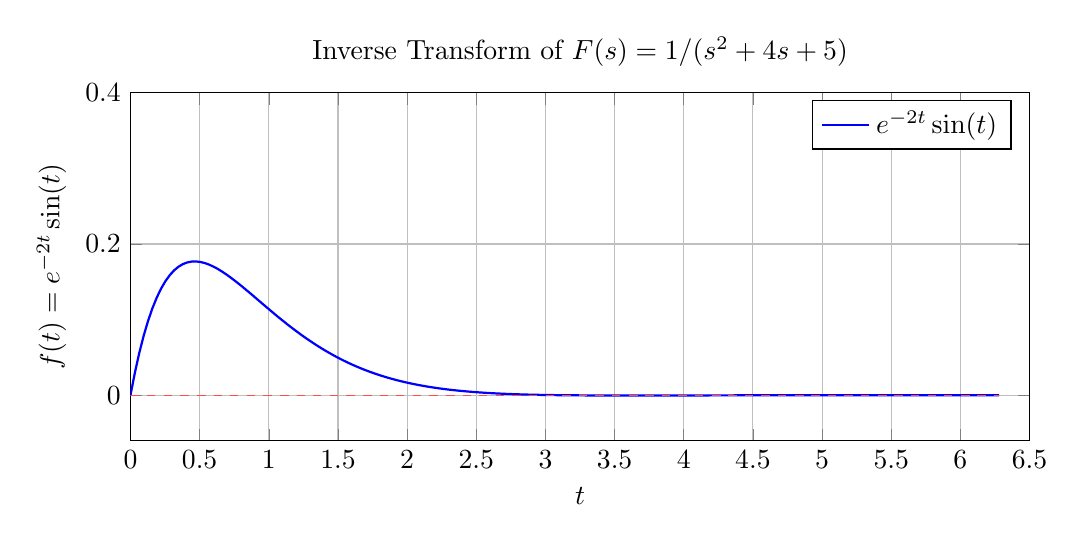
\begin{tikzpicture}
\begin{axis}[
  xlabel={$t$}, ylabel={$f(t) = e^{-2t}\sin(t)$},
  xmin=0, xmax=6.5, ymin=-0.06, ymax=0.4,
  domain=0:6.28, samples=200,
  grid=major,
  title={Inverse Transform of $F(s)=1/(s^2+4s+5)$},
  width=13cm, height=6cm
]
\addplot[blue, thick] {exp(-2*x)*sin(deg(x))};
\addlegendentry{$e^{-2t}\sin(t)$}
\addplot[red!70, dashed, domain=0:6.28, samples=200] {0};
\end{axis}
\end{tikzpicture}

\noindent This is the time-domain function corresponding to
$F(s) = 1/(s^2+4s+5)$ --- a damped sinusoidal response, typical of
underdamped systems. The amplitude decays exponentially as $e^{-2t}$ while
oscillating at unit frequency.

\subsection*{Plot 2: $f(t) = t\,e^{3t}$ --- Exponential Growth}

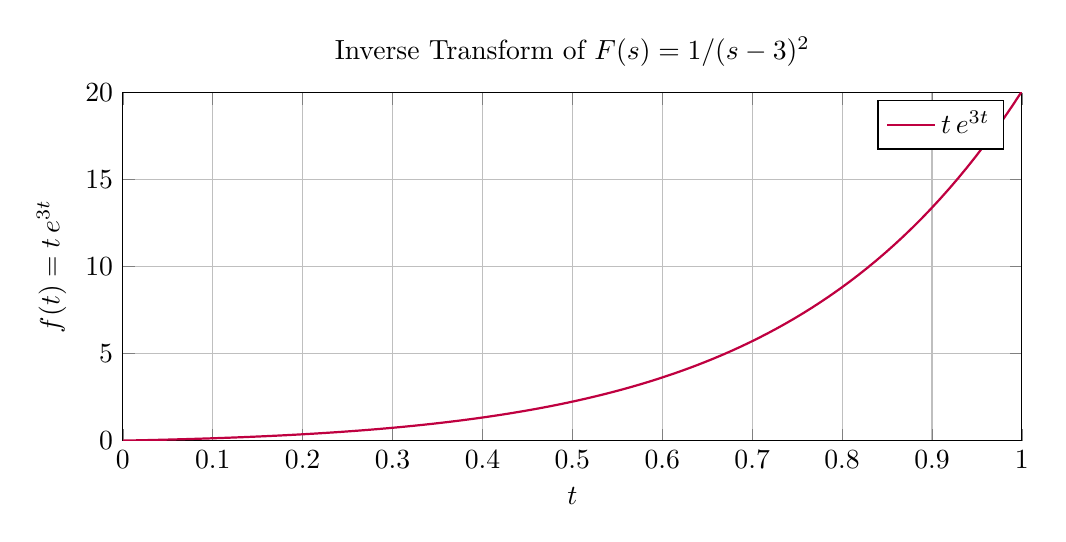
\begin{tikzpicture}
\begin{axis}[
  xlabel={$t$}, ylabel={$f(t) = t\,e^{3t}$},
  xmin=0, xmax=1, ymin=0, ymax=20,
  domain=0:1, samples=100,
  grid=major,
  title={Inverse Transform of $F(s)=1/(s-3)^2$},
  width=13cm, height=6cm
]
\addplot[purple, thick] {x*exp(3*x)};
\addlegendentry{$t\,e^{3t}$}
\end{axis}
\end{tikzpicture}

\noindent This is the time-domain function corresponding to
$F(s) = 1/(s-3)^2$, showing rapid exponential growth. Such responses
appear in unstable systems where the s-domain pole lies in the right
half-plane.

% ======================================================
\section{Worked Examples}

\begin{infobox}{Example 1: Linearity and the Standard Table}
Find $\mathcal{L}^{-1}\!\left\{\dfrac{3}{s} + \dfrac{2}{s^3} - \dfrac{5}{s+4}\right\}$.

\textbf{Step 1 --- Apply linearity.}
\[
  \mathcal{L}^{-1}\!\left\{\frac{3}{s}+\frac{2}{s^3}-\frac{5}{s+4}\right\}
  = 3\,\mathcal{L}^{-1}\!\left\{\frac{1}{s}\right\}
  + 2\,\mathcal{L}^{-1}\!\left\{\frac{1}{s^3}\right\}
  - 5\,\mathcal{L}^{-1}\!\left\{\frac{1}{s+4}\right\}.
\]

\textbf{Step 2 --- Look up each term in the standard table.}
\begin{itemize}
  \item $\mathcal{L}^{-1}\!\left\{\dfrac{1}{s}\right\} = 1$.
  \item $\mathcal{L}^{-1}\!\left\{\dfrac{1}{s^3}\right\} = \dfrac{t^2}{2!} = \dfrac{t^2}{2}$
        (using $1/s^n \to t^{n-1}/(n-1)!$ with $n=3$).
  \item $\mathcal{L}^{-1}\!\left\{\dfrac{1}{s+4}\right\} = e^{-4t}$
        (using $1/(s-a) \to e^{at}$ with $a=-4$).
\end{itemize}

\textbf{Step 3 --- Combine.}
\[
  \mathcal{L}^{-1}\!\left\{\frac{3}{s}+\frac{2}{s^3}-\frac{5}{s+4}\right\}
  = 3\cdot 1 + 2\cdot\frac{t^2}{2} - 5\,e^{-4t}
  = 3 + t^2 - 5\,e^{-4t}.
\]
\end{infobox}

\begin{learnbox}{What Did We Learn?}
Linearity lets you invert term by term. For $1/s^n$, the formula
$t^{n-1}/(n-1)!$ works for all $n\geq 1$. For $1/(s+4)$, read the shift
as $a = -4$ and apply $e^{at}$.
\end{learnbox}

\begin{infobox}{Example 2: Matching Shifted Standard Forms}
Find $\mathcal{L}^{-1}\!\left\{\dfrac{2s+1}{(s-1)^2+4}\right\}$.

\textbf{Step 1 --- Split the numerator to match standard entries.}
Write $2s+1$ in terms of $(s-1)$:
\[
  2s+1 = 2(s-1) + 2 + 1 = 2(s-1) + 3.
\]
So
\[
  \frac{2s+1}{(s-1)^2+4} = \frac{2(s-1)}{(s-1)^2+4} + \frac{3}{(s-1)^2+4}.
\]

\textbf{Step 2 --- Identify base forms and shifts.}
\begin{itemize}
  \item $\dfrac{2(s-1)}{(s-1)^2+4}$: matches $\dfrac{2u}{u^2+4}$ with $u=s-1$,
        i.e.~$2\cdot\dfrac{u}{u^2+2^2}$. Inverse: $\mathcal{L}^{-1}\!\left\{\dfrac{u}{u^2+4}\right\} = \cos(2t)$.
        With shift $a=1$: gives $2\,e^{t}\cos(2t)$.
  \item $\dfrac{3}{(s-1)^2+4}$: matches $\dfrac{3}{u^2+2^2}$.
        Write as $\dfrac{3}{2}\cdot\dfrac{2}{u^2+2^2}$.
        Inverse: $\dfrac{3}{2}\,\mathcal{L}^{-1}\!\left\{\dfrac{2}{u^2+4}\right\} = \dfrac{3}{2}\sin(2t)$.
        With shift $a=1$: gives $\dfrac{3}{2}\,e^{t}\sin(2t)$.
\end{itemize}

\textbf{Step 3 --- Combine.}
\[
  \mathcal{L}^{-1}\!\left\{\frac{2s+1}{(s-1)^2+4}\right\}
  = e^{t}\!\left(2\cos(2t) + \frac{3}{2}\sin(2t)\right).
\]
\end{infobox}

\begin{learnbox}{What Did We Learn?}
When a numerator contains $s$ and the denominator is $(s-a)^2+\omega^2$,
always rewrite the numerator as a multiple of $(s-a)$ plus a remainder.
This splits the fraction cleanly into a cosine-type and a sine-type term.
\end{learnbox}

\begin{infobox}{Example 3: Completing the Square in the Denominator}
Find $\mathcal{L}^{-1}\!\left\{\dfrac{s+3}{s^2+6s+13}\right\}$.

\textbf{Step 1 --- Complete the square in the denominator.}
\[
  s^2+6s+13 = (s+3)^2 + 4.
\]

\textbf{Step 2 --- Rewrite the expression.}
\[
  \frac{s+3}{s^2+6s+13} = \frac{s+3}{(s+3)^2+4}.
\]

\textbf{Step 3 --- Match to base form with shift.}
Let $u = s+3$ (i.e.~$a=-3$). Then
\[
  \frac{s+3}{(s+3)^2+4} = \frac{u}{u^2+2^2},
\]
which matches $\dfrac{u}{u^2+\omega^2}$ with $\omega=2$.

\textbf{Step 4 --- Apply the inverse transform.}
\[
  \mathcal{L}^{-1}\!\left\{\frac{u}{u^2+4}\right\} = \cos(2t).
\]
With shift $a=-3$:
\[
  \mathcal{L}^{-1}\!\left\{\frac{s+3}{s^2+6s+13}\right\}
  = e^{-3t}\cos(2t).
\]
\end{infobox}

\begin{learnbox}{What Did We Learn?}
When the numerator exactly matches the form $(s-\alpha)$ after completing
the square, the result is a pure cosine shifted by $e^{\alpha t}$. No
fractional splitting is needed --- the numerator is already in the right form.
\end{learnbox}

% ======================================================
\section{Excel Example (Numerical Verification)}

We verify the inverse transform $f(t) = e^{-2t}\sin(t)$ numerically by
confirming that the Laplace integral $\int_0^\infty e^{-st} f(t)\,dt$
evaluated at $s = 3$ gives $F(3) = 1/(9+12+5) = 1/26 \approx 0.0385$.

\begin{center}
\begin{tabular}{@{}ccccc@{}}
\toprule
Row & \textbf{A: $t$} & \textbf{B: $f(t)=e^{-2t}\sin(t)$}
    & \textbf{C: integrand $e^{-3t}f(t)$} & \textbf{D: Cumulative trap.~sum} \\
\midrule
1   & 0.0  & 0.000000 & 0.000000 & 0.000000 \\
2   & 0.1  & 0.081737 & 0.060552 & 0.003028 \\
3   & 0.2  & 0.133172 & 0.073086 & 0.009710 \\
4   & 0.3  & 0.162185 & 0.065939 & 0.016661 \\
$\vdots$ & $\vdots$ & $\vdots$ & $\vdots$ & $\vdots$ \\
80  & 7.9  & $\approx 0$ & $\approx 0$ & $\approx 0.0385$ \\
\bottomrule
\end{tabular}
\end{center}

\noindent\textbf{Column formulas (starting at row 2, $t$ in column A):}
\begin{itemize}
  \item Column A (time steps, 0 to 8 in steps of 0.1): Row 1 $= 0$;
        subsequent rows $= \texttt{A}(n-1)+0.1$.
  \item Column B: \texttt{=EXP(-2*A2)*SIN(A2)}
  \item Column C (integrand for $s=3$): \texttt{=EXP(-3*A2)*EXP(-2*A2)*SIN(A2)}
        which simplifies to \texttt{=EXP(-5*A2)*SIN(A2)}
  \item Column D (cumulative trapezoidal sum): Row 1 $= 0$;
        rows $\geq 2$: \texttt{=D1+(C1+C2)/2*0.1}
\end{itemize}
In row 80 (at $t = 7.9$), the cumulative sum converges to approximately
$0.0385$, matching the exact value $F(3)=1/26 \approx 0.03846$ to four
decimal places.

\begin{learnbox}{What Did We Learn?}
The trapezoidal rule confirms numerically that $\int_0^\infty e^{-3t}e^{-2t}\sin(t)\,dt \approx 0.0385 = 1/26$.
This validates $\mathcal{L}^{-1}\{1/(s^2+4s+5)\}= e^{-2t}\sin(t)$ beyond
the symbolic table lookup. The integrand decays rapidly because the combined
exponential $e^{-5t}$ forces the integrand to zero well before $t=8$.
\end{learnbox}

% ======================================================
\section{Python Example}

\begin{lstlisting}[language=Python, caption={Symbolic Inverse Laplace Transforms with SymPy}]
import sympy as sp

s, t = sp.symbols('s t')

# --- Example 1 ---
F1 = sp.Rational(3,1)/s + sp.Rational(2,1)/s**3 - sp.Rational(5,1)/(s+4)
f1 = sp.inverse_laplace_transform(F1, s, t)
print("Example 1:", sp.simplify(f1))
# Expected: 3 + t**2 - 5*exp(-4*t)  (for t >= 0)

# Verify by forward transform
F1_check = sp.laplace_transform(f1, t, s, noconds=True)
print("Verify Example 1 F(s):", sp.simplify(F1_check - F1) == 0)
# Expected: True

# --- Example 2 ---
F2 = (2*s + 1) / ((s-1)**2 + 4)
f2 = sp.inverse_laplace_transform(F2, s, t)
print("Example 2:", sp.simplify(f2))
# Expected: exp(t)*(2*cos(2*t) + (3/2)*sin(2*t))  (for t >= 0)

# Verify
F2_check = sp.laplace_transform(f2, t, s, noconds=True)
print("Verify Example 2 F(s):", sp.simplify(F2_check - F2) == 0)
# Expected: True

# --- Example 3 ---
F3 = (s + 3) / (s**2 + 6*s + 13)
f3 = sp.inverse_laplace_transform(F3, s, t)
print("Example 3:", sp.simplify(f3))
# Expected: exp(-3*t)*cos(2*t)  (for t >= 0)

# Verify
F3_check = sp.laplace_transform(f3, t, s, noconds=True)
print("Verify Example 3 F(s):", sp.simplify(F3_check - F3) == 0)
# Expected: True
\end{lstlisting}

\begin{learnbox}{What Did We Learn?}
SymPy's \texttt{inverse\_laplace\_transform} handles all three techniques
automatically. Re-applying the forward transform and checking that the
difference is zero gives a clean symbolic verification. This workflow ---
compute inverse, verify forward --- is a reliable sanity-check for any
inverse transform computation.
\end{learnbox}

% ======================================================
\section{Viva-Style Oral Questions}

\begin{enumerate}

\item \textbf{Q: Define the inverse Laplace transform.}\\
\textbf{A:} If $\mathcal{L}\{f(t)\} = F(s)$, then the inverse Laplace transform
is $\mathcal{L}^{-1}\{F(s)\} = f(t)$. It returns a function of $t$ whose
Laplace transform is the given $F(s)$.

\item \textbf{Q: State Lerch's theorem and explain its significance.}\\
\textbf{A:} Lerch's theorem states that if two piecewise continuous functions
$f_1(t)$ and $f_2(t)$ on $[0,\infty)$ have the same Laplace transform
$F(s)$, then $f_1(t) = f_2(t)$ at every point of continuity. Its
significance: the inverse transform is unique among piecewise continuous
functions, so the table-lookup approach is unambiguous.

\item \textbf{Q: What is the Bromwich integral and why is it not used directly in
this course?}\\
\textbf{A:} The Bromwich (Mellin--Fourier) integral is
$f(t) = \frac{1}{2\pi i}\int_{c-i\infty}^{c+i\infty}e^{st}F(s)\,ds$.
It is the rigorous inversion formula but requires contour integration in the
complex plane (residues, etc.), which is beyond the scope of this B.Tech
course. Instead, we use the inverse transform table and algebraic techniques.

\item \textbf{Q: State the linearity property of the inverse Laplace transform.}\\
\textbf{A:} For constants $a$ and $b$:
$\mathcal{L}^{-1}\{aF(s)+bG(s)\} = a\,\mathcal{L}^{-1}\{F(s)\}+b\,\mathcal{L}^{-1}\{G(s)\}$.
This follows directly from the linearity of the forward transform.

\item \textbf{Q: How do you use the inverse first shifting theorem?}\\
\textbf{A:} If $\mathcal{L}^{-1}\{F(s)\}=f(t)$, then
$\mathcal{L}^{-1}\{F(s-a)\}=e^{at}f(t)$. In practice: identify the shift
$a$, strip it to obtain the base form $F(s)$, look up $f(t) = \mathcal{L}^{-1}\{F(s)\}$
from the table, then multiply by $e^{at}$.

\item \textbf{Q: When and why do we complete the square?}\\
\textbf{A:} We complete the square when the denominator is an irreducible
quadratic $s^2+bs+c$ that cannot be factored over the reals. The technique
converts it to $(s-\alpha)^2+\omega^2$, enabling a direct match to the
sinusoidal entries in the inverse table combined with the shift theorem.

\item \textbf{Q: Give the inverse transforms of $1/s$, $1/s^2$, and $1/(s^2+a^2)$.}\\
\textbf{A:}
$\mathcal{L}^{-1}\{1/s\}=1$; \quad
$\mathcal{L}^{-1}\{1/s^2\}=t$; \quad
$\mathcal{L}^{-1}\!\left\{\dfrac{1}{s^2+a^2}\right\}=\dfrac{1}{a}\sin(at)$\; (since $\mathcal{L}^{-1}\{a/(s^2+a^2)\}=\sin(at)$).

\item \textbf{Q: What notation distinguishes the forward and inverse Laplace transforms?}\\
\textbf{A:} $\mathcal{L}$ denotes the forward (direct) Laplace transform:
$f(t)\mapsto F(s)$. $\mathcal{L}^{-1}$ denotes the inverse Laplace transform:
$F(s)\mapsto f(t)$. These must never be confused; using the wrong symbol
reverses the direction of the operation.

\end{enumerate}

% ======================================================
\section{Descriptive Questions}

\begin{enumerate}

\item \textbf{Define the inverse Laplace transform and state Lerch's theorem.}\\
Write a complete answer covering: (i) the definition $\mathcal{L}^{-1}\{F(s)\}=f(t)$
means $f(t)$ is the function whose Laplace transform is $F(s)$;
(ii) the Bromwich integral as the formal inversion formula;
(iii) Lerch's theorem: uniqueness among piecewise continuous functions on
$[0,\infty)$; (iv) why uniqueness justifies the table-based approach.

\item \textbf{Prove that the inverse Laplace transform is linear.}\\
Let $\mathcal{L}^{-1}\{F(s)\}=f(t)$ and $\mathcal{L}^{-1}\{G(s)\}=g(t)$.
By linearity of $\mathcal{L}$:
$\mathcal{L}\{af(t)+bg(t)\}=a\mathcal{L}\{f(t)\}+b\mathcal{L}\{g(t)\}=aF(s)+bG(s)$.
Applying $\mathcal{L}^{-1}$: $\mathcal{L}^{-1}\{aF(s)+bG(s)\}=af(t)+bg(t)$.
This proof is complete.

\item \textbf{Find $\mathcal{L}^{-1}\!\left\{\dfrac{2s+3}{s^2+4s+7}\right\}$ step by step.}\\
(i) Complete the square: $s^2+4s+7=(s+2)^2+3$.
(ii) Split the numerator: $2s+3=2(s+2)-4+3=2(s+2)-1$.
(iii) Write: $\dfrac{2(s+2)-1}{(s+2)^2+3}=\dfrac{2(s+2)}{(s+2)^2+3}-\dfrac{1}{(s+2)^2+3}$.
(iv) Match and apply shift ($a=-2$, $\omega=\sqrt{3}$):
$2e^{-2t}\cos(\sqrt{3}\,t)-\dfrac{1}{\sqrt{3}}e^{-2t}\sin(\sqrt{3}\,t)$.

\item \textbf{State and apply the inverse first shifting theorem.}\\
State: if $\mathcal{L}^{-1}\{F(s)\}=f(t)$ then $\mathcal{L}^{-1}\{F(s-a)\}=e^{at}f(t)$.
Application: find $\mathcal{L}^{-1}\!\left\{1/(s-2)^4\right\}$.
Base form $F(s)=1/s^4$: $\mathcal{L}^{-1}=t^3/6$. Shift $a=2$:
$\mathcal{L}^{-1}\!\left\{1/(s-2)^4\right\}=\dfrac{t^3}{6}e^{2t}$.

\item \textbf{Explain the relationship between the forward and inverse tables.}\\
The forward table lists $f(t) \to F(s)$. Reading the same table in reverse
gives the inverse table $F(s) \to f(t)$. Both tables carry identical
information; the direction of lookup is all that changes. Lerch's theorem
guarantees that the reverse lookup is unambiguous for piecewise continuous
functions. In practice, every entry learned in Unit IV is automatically
an entry in the Unit V inverse table.

\end{enumerate}

% ======================================================
\section{Practice Problems}

\begin{enumerate}

\item Find $\mathcal{L}^{-1}\!\left\{\dfrac{4}{s^3}\right\}$.\\
\textit{Hint:} Use $1/s^n \to t^{n-1}/(n-1)!$ with $n=3$.\\
\textit{Answer:} $2t^2$.

\item Find $\mathcal{L}^{-1}\!\left\{\dfrac{1}{s^2-9}\right\}$.\\
\textit{Hint:} Write as $\dfrac{1}{(s-3)(s+3)}$ and use $\sinh(at)/a \leftrightarrow 1/(s^2-a^2)$
or partial fractions.\\
\textit{Answer:} $\dfrac{1}{3}\sinh(3t)$.

\item Find $\mathcal{L}^{-1}\!\left\{\dfrac{s}{s^2+4s+8}\right\}$.\\
\textit{Hint:} Complete the square: $s^2+4s+8=(s+2)^2+4$.
Split $s = (s+2)-2$.\\
\textit{Answer:} $e^{-2t}\!\left(\cos(2t) - \sin(2t)\right)$.

\item Find $\mathcal{L}^{-1}\!\left\{\dfrac{3}{(s-2)^4}\right\}$.\\
\textit{Hint:} Use $1/s^4 \to t^3/6$, then shift $a=2$.\\
\textit{Answer:} $\dfrac{t^3}{2}\,e^{2t}$.

\item Find $\mathcal{L}^{-1}\!\left\{\dfrac{e^{-2s}}{s}\right\}$.\\
\textit{Hint:} $e^{-as}/s \to u(t-a)$ from the standard table.\\
\textit{Answer:} $u(t-2)$ (unit step shifted to $t=2$).

\item Find $\mathcal{L}^{-1}\!\left\{\dfrac{s+1}{s^2+2s+5}\right\}$.\\
\textit{Hint:} Complete the square: $s^2+2s+5=(s+1)^2+4$.
Numerator $s+1$ matches $(s-(-1))$ exactly.\\
\textit{Answer:} $e^{-t}\cos(2t)$.

\end{enumerate}

% ======================================================
\section{MCQs}

\begin{enumerate}

\item If $\mathcal{L}\{f(t)\} = F(s)$, then $\mathcal{L}^{-1}\{F(s)\}$ equals:\\
(a) $F(t)$ \quad (b) $f(-t)$ \quad \textbf{(c) $f(t)$} \quad (d) $F(-s)$\\
\textit{Explanation:} By definition, $\mathcal{L}^{-1}$ inverts the Laplace transform,
returning the original time-domain function $f(t)$.

\item Lerch's theorem guarantees that the inverse Laplace transform is:\\
(a) Always zero for $t < 0$ \quad (b) Differentiable everywhere \quad
\textbf{(c) Unique among piecewise continuous functions} \quad
(d) Defined only for rational $F(s)$\\
\textit{Explanation:} Lerch's theorem ensures uniqueness among piecewise
continuous functions on $[0,\infty)$, making the table-lookup unambiguous.

\item $\mathcal{L}^{-1}\!\left\{\dfrac{1}{s}\right\}$ equals:\\
(a) $t$ \quad \textbf{(b) $1$} \quad (c) $e^t$ \quad (d) $\delta(t)$\\
\textit{Explanation:} From the standard table, $\mathcal{L}\{1\} = 1/s$,
so $\mathcal{L}^{-1}\{1/s\} = 1$.

\item The inverse first shifting theorem states $\mathcal{L}^{-1}\{F(s-a)\}$ equals:\\
(a) $f(t-a)$ \quad (b) $f(t)u(t-a)$ \quad \textbf{(c) $e^{at}f(t)$}
\quad (d) $e^{-at}f(t)$\\
\textit{Explanation:} Shifting the argument from $s$ to $s-a$ in the
s-domain corresponds to multiplication by $e^{at}$ in the time domain.

\item Completing the square in the denominator is used to:\\
(a) Simplify the numerator polynomial \quad
(b) Convert the transform to partial fractions \quad
\textbf{(c) Match the quadratic denominator to the standard sinusoidal forms}
\quad (d) Eliminate complex roots\\
\textit{Explanation:} Completing the square converts $s^2+bs+c$ to
$(s-\alpha)^2+\omega^2$, enabling a direct match to the $\sin(\omega t)$
or $\cos(\omega t)$ entries in the inverse table via the shift theorem.

\end{enumerate}

% ======================================================
\section{Common Mistakes}

\begin{mistakebox}{Common Mistakes in Inverse Laplace Transforms}
\begin{tabular}{@{}p{4cm}p{5cm}p{5.5cm}@{}}
\toprule
\textbf{Mistake} & \textbf{What Students Do} & \textbf{Correct Approach} \\
\midrule
Confusing $\mathcal{L}$ with $\mathcal{L}^{-1}$ &
  Write $\mathcal{L}$ when inverting, or apply the forward table in the wrong direction &
  Always write $\mathcal{L}^{-1}\{F(s)\}$ when going from $s$-domain to $t$-domain \\
\addlinespace
Skipping completing the square &
  Try to invert $1/(s^2+4s+5)$ directly by guessing or wrong factoring &
  First complete the square: $s^2+4s+5=(s+2)^2+1$; then match \\
\addlinespace
Matching $1/(s^2+a^2)$ to $\sin(at)$ incorrectly &
  Write $\mathcal{L}^{-1}\{1/(s^2+a^2)\}=\sin(at)$ without checking the numerator &
  The correct entry is $\mathcal{L}^{-1}\{a/(s^2+a^2)\}=\sin(at)$; the numerator must be $a$, not $1$ \\
\addlinespace
Applying the shift to only part of the expression &
  When finding $\mathcal{L}^{-1}\{F(s-a)\}$, substitute $s-a$ into the formula but forget to replace every occurrence of $s$ &
  Replace $s$ by $s-a$ everywhere in $F(s)$ before looking up the base form \\
\addlinespace
Assuming $\mathcal{L}^{-1}\{F(s)G(s)\}=f(t)g(t)$ &
  Multiply the two inverse transforms directly &
  The correct result is the convolution $(f*g)(t)=\int_0^t f(\tau)g(t-\tau)\,d\tau$ (covered in Topic 04) \\
\bottomrule
\end{tabular}
\end{mistakebox}

% ======================================================
\section{Quick Recap}

\begin{learnbox}{Quick Recap --- Topic 01: Inverse Laplace Transform}
\begin{itemize}
  \item $\mathcal{L}^{-1}\{F(s)\}=f(t)$ is the function whose Laplace transform
        is $F(s)$ --- it is the ``undo'' operation.
  \item The formal inversion is the Bromwich integral; in practice, use the
        inverse table and algebraic techniques.
  \item \textbf{Lerch's theorem}: the inverse is unique among piecewise
        continuous functions on $[0,\infty)$.
  \item \textbf{Linearity}: $\mathcal{L}^{-1}\{aF(s)+bG(s)\}=af(t)+bg(t)$
        --- invert term by term.
  \item \textbf{Standard inverse table}: 10 core entries covering powers,
        exponentials, sinusoids, hyperbolic functions, unit step, and delta.
  \item \textbf{Inverse first shifting theorem}:
        $\mathcal{L}^{-1}\{F(s-a)\}=e^{at}f(t)$ --- a shift in $s$ by $a$
        multiplies $f(t)$ by $e^{at}$.
  \item \textbf{Completing the square}: converts $s^2+bs+c$ to
        $(s-\alpha)^2+\omega^2$, enabling direct match to sinusoidal table entries.
  \item Up next (Topic 02): the full inverse table for elementary functions;
        Topics 03--04: partial fractions and convolution for complex $F(s)$.
\end{itemize}
\end{learnbox}

\end{document}
